\section{Teori} \label{sec:Lieth_Wahid-theory}
I detta avsnitt presenteras bakgrunder och teorier som är relevanta till undersökningen. 
\subsection{Vattenfall}
Vattenfall är den mest använda utvecklingsmetodiken inom mjukvarurelaterade högskolekurser. Metoden introducerades i 1970-talet \cite{WaterfalM} av Dr. Winston W. Royce. \cite{managing} Vattenfall är en sekventiell utvecklingsprocess. Det vill säga att all utveckling sker på ett sekventiellt sätt vilket innebär mindre flexibilitet. Figur \ref{Vattenfallsmodellen} visar de typiska 
stegen som en denna modell följer. Metoden är uppdelad i olika faser och eftersom allt sker sekventiellt innebär detta att varje fas måste vara avklarad innan den nästa kan börja.  I början av kedjan kommer kravspecifikation under vilken genereras alla relevanta dokumenten som sedan kommer vara avtalet mellan kunden och utvecklingsteamet. \cite{GameDesign} Därefter kommer designfasen under vilken ett detaljerat designdokument produceras. Därefter kommer Implementationfasen under vilken börjar implementationsprocessen. Därefter kommer veriferingsfasen under vilken valideras programmets funktionalitet och eventuellt kommer testfasen under vilken programmet testas och säkerställs att den möter kravspecifikationen.
\begin{figure*}[h]
	\centering
	\includegraphics[scale=0.8]{VF}
	\caption{Vattenfallsmodellen\cite{theWaterFall}}
	\label{Vattenfallsmodellen}
\end{figure*}
\subsection{Scrum}
Scrum är ett de mest populära ramverken inom agil mjukvaruutveckling. Ramverket utvecklades i mitten av 1990-talet av Jeff Sutherland, John Scumniotales och Jeff McKenna Det är möjligt att Scrum viktigaste egenskap är dess så kallad iterativa process som tillåter förändringar att hända när det behövs. Under utvecklingsprocessen, Scrum, deltagare av ett utvecklingsteam jobbar ihop för att föra projektet framåt genom att använda s.k. Scrum artefakter som t.ex. \textit{produkt-backlog} och \textit{sprint-backlog}. Detta möjliggör för teamet att vara medvetna om senaste ändringar i kraven och omprioriterar om sådant behövs.  \cite{aamir2017incorporating} Eftersom Scrum är flexibel och kan ändras sådant att den passar varje grupps behov bestämde vårt team att inte inkludera all delar av Scrum utan bara vissa delar som teamet ansåg vara relevant för arbetet. Dess delar är:
Scrum-bräde, Scrum-möte, och veckorapporter samt burndown-chart. Mer detaljerad beskrivning av Scrum som användes under projektets gång kan återfinnas under. Figur \ref{sp} visar dem typiska stegen som Scrum Utvecklingensmetodiken följer.
\ref{main:Scrum}.
\begin{figure*}[h]
	\centering
	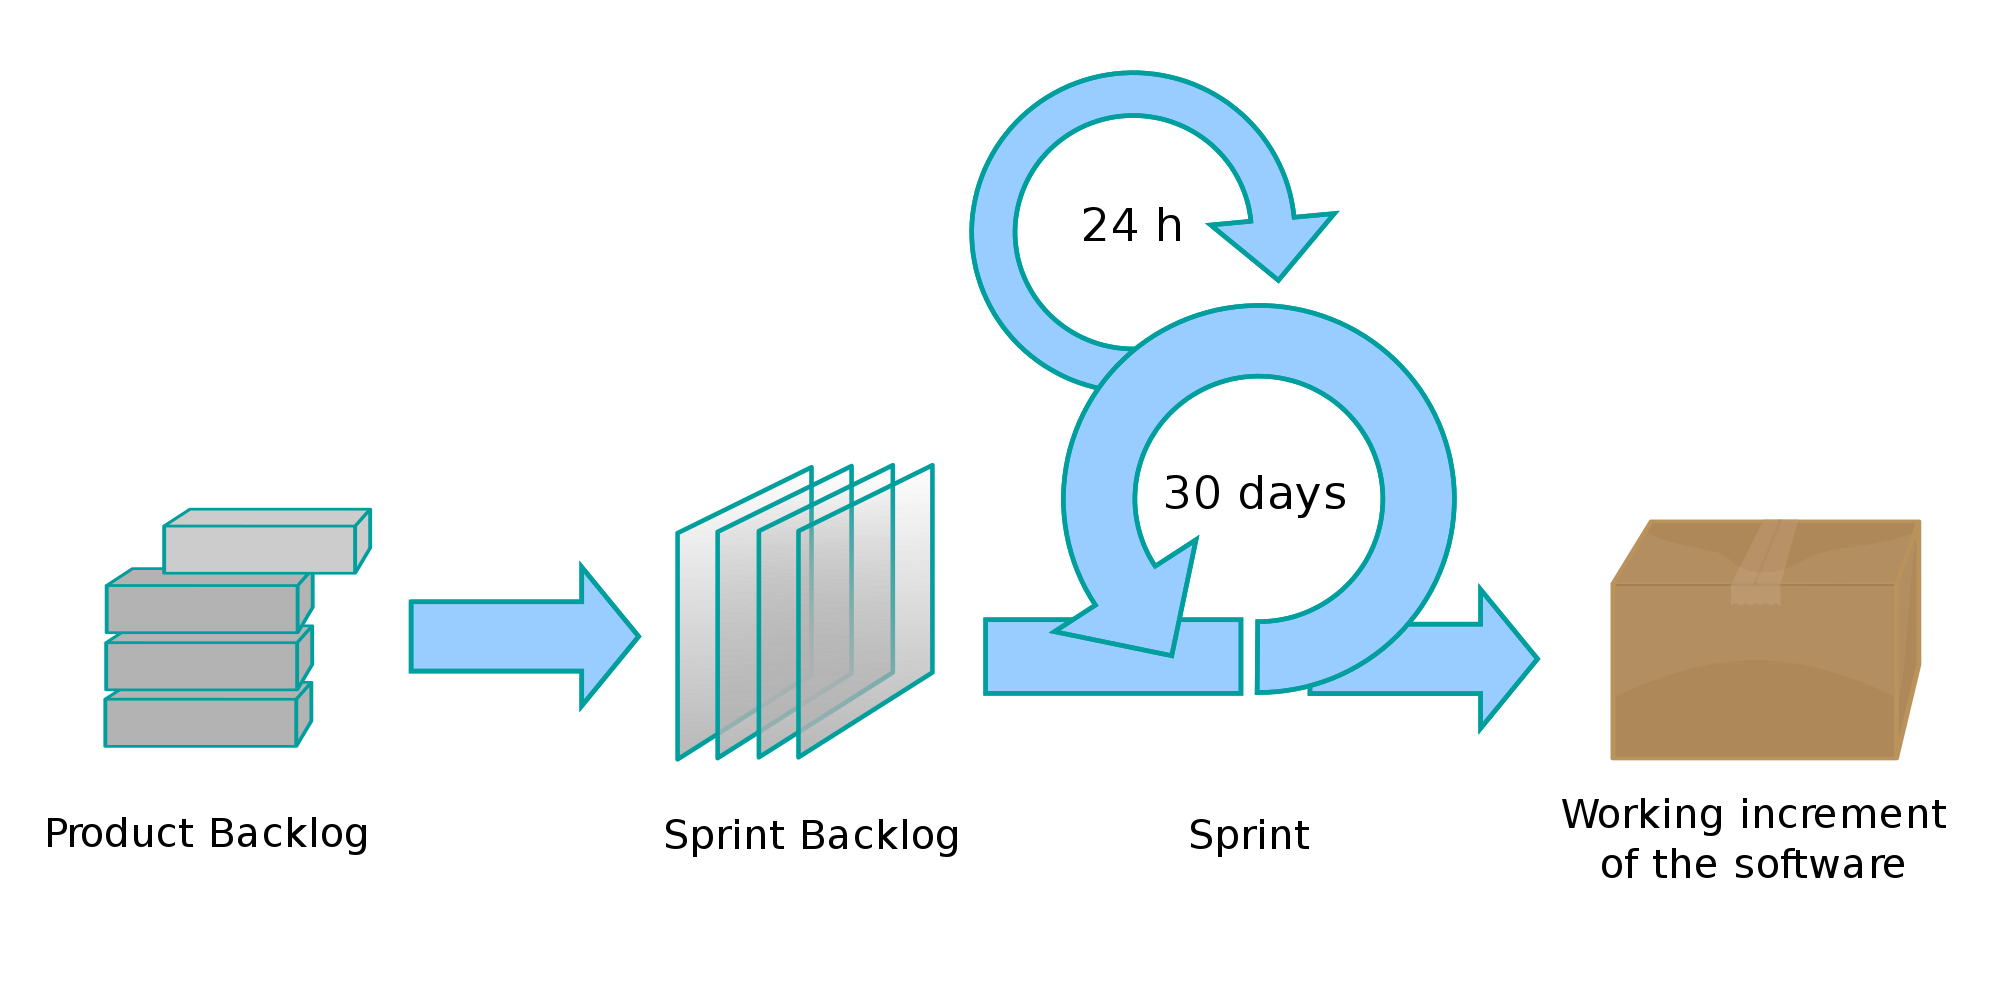
\includegraphics[scale=0.2]{Scp}
	\caption{Dem typiska stegen som följs i Scrum\cite{Scrumprocess}}
	\label{sp}
\end{figure*}
